\section{Accuracy calculation}\label{accuracy_calculation}


In order to estimate the overfill and underfill, we need to accurately calculate the area covered by a single extrusion path.
If we would simply use an isosceles trapezoidal area with base lengths equal to the widths of the two end points of the extrusion segment, we would get artifacts at corners in the toolpath (\cref{segment_visualization}a).
We therefore use a semi-circle (\cref{segment_visualization}b) with a diameter equal to the starting width in the one end of each segment, and exclude it at the other end, because it will be included in the next segment.
For polyline extrusion paths which are not closed, we also include the semi-circle corresponding to the extrusion width of the end-position ( \cref{segment_visualization}c).

%In order to print such extrusion paths accurately, we can modulate the amount of material flow per millimeter based on this visualization model.
%See \cref{segment_visualization}.

\begin{figure}
\centering
\setlength{\figwidth}{.25\columnwidth}
\begin{subfigure}{\figwidth}\centering
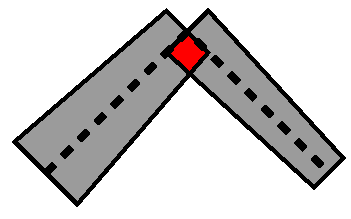
\includegraphics[width=\columnwidth]{sources/validation/visualization_principle_blocky.pdf}
\caption{Blocky}
\end{subfigure}
\begin{subfigure}{\figwidth}\centering
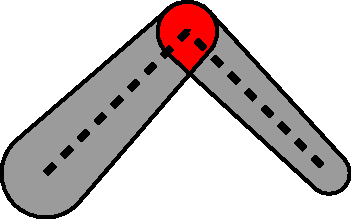
\includegraphics[width=\columnwidth]{sources/validation/visualization_principle_rounded.pdf}
\caption{Rounded}
\end{subfigure}
\begin{subfigure}{\figwidth}\centering
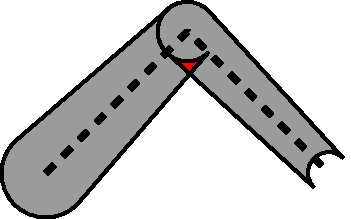
\includegraphics[width=\columnwidth]{sources/validation/visualization_principle_rounded_excluded.pdf}
\caption{Excluded}
\end{subfigure}
\caption{
Extruded area of two extrusion segments.
Red areas signify doubly extruded areas.
}
\label{segment_visualization}
\end{figure}

We can then estimate the amount of underfill by unioning the rounded visualization of all extrusion segments and then taking the difference from the original outline shape.
In order to deal with rounding errors, we perform a morphological close of \SI{5}{\micro\meter} before calculating the total area of the underfill regions.

The overfill regions are calculated by adding the polygonal areas of each extrusion segment to a list.
We then add the original outline shape in reverse and perform a Vatti clipping operation~\cite{Vatti2019clipping} which only keeps areas of positive winding number.
Because the reverse outline shape reduces the winding number of all extruded segments by one, only the overfill areas are left with a positive winding number.
In order to estimate the areas which are triply covered by extrusion segments, we repeat the process of adding the outline in reverse and performing Vatti's clipping operation.
These triple extrusion areas count double toward the total amount of overfill.
The resulting overfill and underfill areas are visualized for the different toolpath schemes in the top of \cref{visualized_accuracy}.

